\chapter{Linking and holomorphic maps}\label{ch:linking}

\section{Linking numbers}\label{sec:lk}

Let $K_1,K_2\subset S^3$ be disjoint oriented closed $1$-manifolds. Since $H_1(S^3)=0$, $K_1$ bounds an oriented surface $\Sigma$ (a Seifert surface, or more generally a $2$-chain), which may be chosen transverse to $K_2$, and the \emph{linking number} $\lk(K_1,K_2)$ is the algebraic intersection number $\Sigma\cdot K_2$. It does not depend on $\Sigma$, it is symmetric, and for $K_1,K_2\subset\R^3$ it is given by the Gauss integral
\begin{equation}\label{eq:gauss}
\lk(K_1,K_2)=\frac1{4\pi}\oint_{K_1}\oint_{K_2}\frac{(\mathbf x-\mathbf y)\cdot(d\mathbf x\times d\mathbf y)}{|\mathbf x-\mathbf y|^3}.
\end{equation}
The integral \eqref{eq:gauss} is used in Appendix~\ref{app:checks} to check the computations of this chapter numerically.

Orient the fibres of $h\colon S^3\to S^2$ by the circle action $\lambda\mapsto(\lambda z,\lambda w)$.

\begin{proposition}\label{prop:fibrelink}
Any two distinct fibres of $h$ have linking number $\varepsilon$, where $\varepsilon\in\{\pm1\}$ depends only on the orientation of $S^3$.
\end{proposition}

\begin{proof}
The fibre over the north pole $N_0$ is $C_\infty=\{(z,0):|z|=1\}$. It bounds the hemisphere
\[
\Sigma=\{(z,t)\in S^3:t\in\R,\ t\ge0\},
\]
a $2$-disc. By Corollary~\ref{cor:fibration} the fibre over $s(x)$, $x\in\C$, is $C_x=\{(xc,c):|c|=(1+|x|^2)^{-1/2}\}$, and it meets $\Sigma$ exactly where $c$ is real and positive, at one point. The intersection is transverse: along $C_x$, written as $c=\rho e^{i\phi}$, the function $\Imag w=\rho\sin\phi$ that cuts out $\Sigma$ near the intersection has nonzero derivative $\rho$ at $\phi=0$. So $\lk(C_\infty,C_x)=\pm1$, and the sign is constant in $x$ because $\C$ is connected and the fibres $C_x$ vary continuously. Now let $C_p,C_q$ be any two distinct fibres. The group $\U(2)$ acts on $S^3$ by orientation-preserving isometries commuting with the circle action, so it permutes the oriented fibres, and it acts transitively on $S^2$ through $\U(2)\to\SO(3)$. Choosing $g\in\U(2)$ with $gC_p=C_\infty$ gives $\lk(C_p,C_q)=\lk(C_\infty,gC_q)$, which is the constant found above.
\end{proof}

The connection with the Hopf invariant is Hopf's original definition \cite{Hop31}; see \cite[Section~17]{BT82} for a proof.

\begin{theorem}[Linking formula]\label{thm:linkingformula}
Let $f\colon S^3\to S^2$ be smooth and let $p\neq q$ be regular values. Orient $f^{-1}(p)$ and $f^{-1}(q)$ as preimages. Then $\Hopf(f)=\pm\lk(f^{-1}(p),f^{-1}(q))$, with a universal sign.
\end{theorem}

We fix the orientation of $S^3$ (the boundary orientation of the unit ball in $\C^2$ with its complex orientation) and choose the generators in Definition~\ref{def:hopfinv} so that $\Hopf(h)=1$. With these choices the universal sign is $\varepsilon$, by Proposition~\ref{prop:fibrelink} applied to $f=h$: the fibres of $h$, oriented by the circle action, are its preimages with their preimage orientation up to one fixed sign.

\begin{figure}[t]
\centering
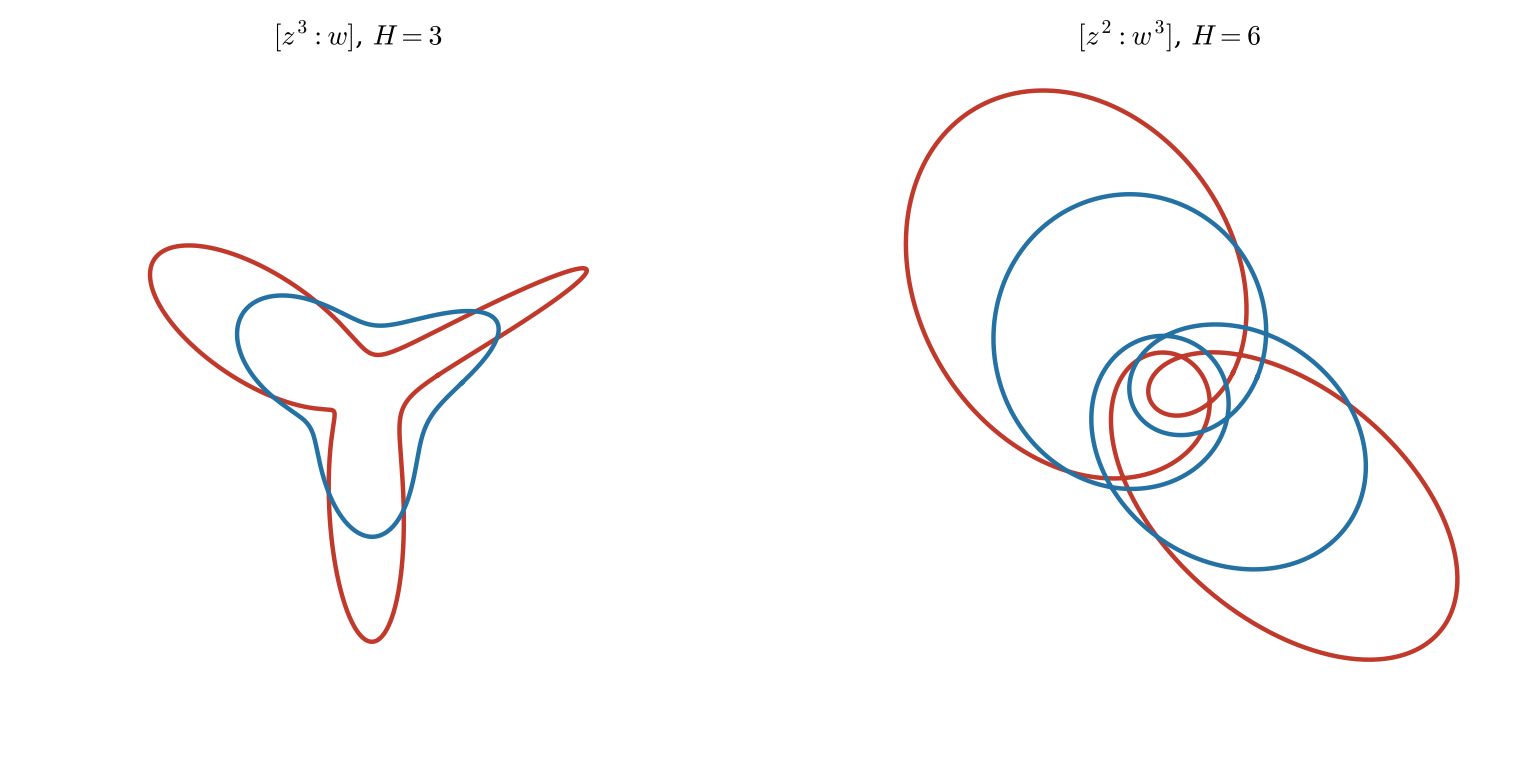
\includegraphics[width=0.95\textwidth]{fig_torus_links.png}
\caption{Two fibres of $[z^3:w]$, with Hopf invariant $3$ (left), and of $[z^2:w^3]$, with Hopf invariant $6$ (right), after stereographic projection. Each fibre lies on a torus about the axis and is a torus link of type $(p,q)$; the Gauss integral \eqref{eq:gauss} gives linking numbers $3$ and $6$ (Appendix~\ref{app:checks}).}
\label{fig:toruslinks}
\end{figure}

\section{Holomorphic maps}\label{sec:holomorphic}

Let $P,Q\in\C[z,w]$ have no common zero on $S^3$, put $F=(P,Q)\colon\C^2\to\C^2$ and
\[
[P:Q]=h\circ\frac{F}{|F|}\colon S^3\to S^2 ,
\]
which is the map $u\mapsto[P(u):Q(u)]\in\CP^1=S^2$ in the chart \eqref{eq:stereo} with $x=P/Q$; the formula of the Introduction follows from $h(\lambda v)=\lambda^2h(v)$ for real $\lambda$. Let $Z=\{u\in\C^2:P(u)=Q(u)=0\}$.

\begin{lemma}\label{lem:bounded}
Let $C\subset\C^2$ be an irreducible affine plane curve that does not meet $S^3$. Then $C$ does not meet the closed ball $\bar B^4$.
\end{lemma}

\begin{proof}
The closure of $C$ in $\CP^2$ is an irreducible projective curve, and $C$ is its complement of the finitely many points at infinity, so $C$ is connected in the classical topology \cite[Corollary~(4.16)]{Mum76}. As $C\cap S^3=\emptyset$, $C$ is the disjoint union of the open sets $C\cap B^4$ and $C\setminus\bar B^4$, so if $C$ meets $\bar B^4$ then $C\subset B^4$ is bounded. But no affine curve $C=\{D=0\}$, $D$ irreducible, is bounded. If $D$ has degree $k\ge1$ in $w$, with leading coefficient $a(z)$, then for every $z_1$ with $a(z_1)\neq0$ the polynomial $D(z_1,\cdot)$ has a root, so the projection of $C$ to the $z$-coordinate contains the complement of a finite set. If $D$ has degree $0$ in $w$, it is an irreducible polynomial in $z$ alone, that is $D=z-z_0$ up to a scalar, and $C=\{z_0\}\times\C$.
\end{proof}

\begin{lemma}[Finiteness]\label{lem:finite}
Let $D=\gcd(P,Q)$ and $P=DP'$, $Q=DQ'$. Then $Z\cap\bar B^4=\{P'=Q'=0\}\cap B^4$; this set is finite, and $I_u(P,Q)=I_u(P',Q')$ at each of its points.
\end{lemma}

\begin{proof}
$Z=\{D=0\}\cup\{P'=Q'=0\}$. Every irreducible component of $\{D=0\}$ lies in $Z$, so it does not meet $S^3$, and by Lemma~\ref{lem:bounded} it does not meet $\bar B^4$. The coprime polynomials $P',Q'$ have at most $\deg P'\cdot\deg Q'$ common zeros in $\C^2$ \cite[Section~5.3]{Ful69}, and none on $S^3$. At a point $u$ with $D(u)\neq0$, $D$ is a unit in the local ring $\mathcal O_u$, so $(P,Q)=(P',Q')$ in $\mathcal O_u$.
\end{proof}

\begin{lemma}[Degree as a sum of indices]\label{lem:indexsum}
Let $\Phi\colon\bar B^{n}\to\R^{n}$ be smooth with finitely many zeros, all in the open ball. Then the degree of $\Phi/|\Phi|\colon S^{n-1}\to S^{n-1}$ is the sum of the local indices of $\Phi$ at its zeros, where the index at $u$ is the degree of $\Phi/|\Phi|$ on a small sphere about $u$.
\end{lemma}

\begin{proof}
Remove disjoint small open balls $B_u$ about the zeros. On the compact oriented manifold $X=\bar B^n\setminus\bigcup B_u$ the map $\Phi/|\Phi|$ is defined, and its restriction to $\partial X=S^{n-1}\sqcup\bigsqcup(-\partial B_u)$ has degree zero, because it extends over $X$ \cite[Section~5, Lemma~1]{Mil65}. This is the statement, input (I5).
\end{proof}

\begin{proof}[Proof of Theorem~\ref{thm:D}]
Finiteness is Lemma~\ref{lem:finite}. The map $g=F/|F|\colon S^3\to S^3$ satisfies $[P:Q]=h\circ g$, so by Proposition~\ref{prop:composition}, $\Hopf([P:Q])=\deg(g)\Hopf(h)=\deg g$. By Lemma~\ref{lem:indexsum}, applied to $\Phi=F|_{\bar B^4}$, $\deg g$ is the sum of the indices of $F$ at the points of $Z\cap B^4$. At each such point the index of the holomorphic germ $F$ is the intersection multiplicity $I_u(P,Q)$, input (I5) \cite[Chapter~5]{GH78}, \cite[Chapter~5]{AGV85}.\footnote{When $u$ is a regular zero this is the observation that the real Jacobian of a holomorphic map is $|\det_\C DF|^2>0$, so the index is $+1$; in general one perturbs $F$ to $F-\epsilon$ for a small regular value $\epsilon$, whose $I_u(P,Q)$ preimages near $u$ are all regular.} This proves the formula. The sum is $\ge0$, and by Lemma~\ref{lem:finite} and the affine B\'ezout inequality \cite[Section~5.3]{Ful69},
\[
\sum_{u\in Z\cap B^4}I_u(P,Q)=\sum_{u\in B^4}I_u(P',Q')\le\sum_{u\in\C^2}I_u(P',Q')\le\deg P'\cdot\deg Q'\le\deg P\cdot\deg Q .
\]
For $[z^p:w^q]$ the only common zero is $0$, with $I_0(z^p,w^q)=\dim_\C\C[z,w]/(z^p,w^q)=pq$; for $[1:0]$, or any $[P:Q]$ with $Q$ a nonzero constant, there are none. Since $\pi_3(S^2)\cong\Z$ is detected by $\Hopf$ (Theorem~\ref{thm:C}), $[P:Q]$ is null-homotopic exactly when $Z\cap B^4=\emptyset$, every $I_u$ being at least one. Finally $[z^m:w]$ has Hopf invariant $m$, and for the map $\kappa(z,w)=(\bar z,w)$ of degree $-1$ the composite $[z^m:w]\circ\kappa$ has Hopf invariant $-m$ by Proposition~\ref{prop:composition}.
\end{proof}

The two inequalities in the proof give an exact criterion for the upper bound.

\begin{proposition}[Equality]\label{prop:equality}
Let $p=\deg P$ and $q=\deg Q$, and let $\tilde P,\tilde Q$ be the homogenisations in $\CP^2$. Then $\Hopf([P:Q])=pq$ if and only if $P$ and $Q$ have no common factor, $\tilde P$ and $\tilde Q$ have no common zero on the line at infinity, and all common zeros of $P$ and $Q$ in $\C^2$ lie in $B^4$.
\end{proposition}

\begin{proof}
By B\'ezout's theorem in $\CP^2$ \cite[Section~5.3]{Ful69}, two curves of degrees $p$ and $q$ without common component meet in exactly $pq$ points counted with multiplicity. If $D=\gcd(P,Q)$ is not constant, the chain of inequalities above is strict at the last step. Otherwise the sum over $\C^2$ equals $pq$ minus the multiplicities at infinity, and the sum over $B^4$ equals the sum over $\C^2$ exactly when no common zero lies outside $\bar B^4$; none lies on $S^3$ by hypothesis.
\end{proof}

\begin{example}\label{ex:holoexamples}
\begin{enumerate}[label=\textup{(\alph*)}]
\item $[z^p:w^q]$: $\Hopf=pq$. The fibre over a point $[\alpha:\beta]$ with $\alpha\beta\neq0$ lies on the torus $|z|=r_1$, $|w|=r_2$ determined by $r_1^2+r_2^2=1$ and $r_1^p|\beta|=r_2^q|\alpha|$, and there it is the set $\{p\arg z-q\arg w\equiv\arg(\alpha/\beta)\}$, the torus link of type $(p,q)$ with $\gcd(p,q)$ components. Two such fibres have linking number $pq$, as Theorem~\ref{thm:linkingformula} requires; Figure~\ref{fig:toruslinks} shows the cases $(3,1)$ and $(2,3)$.
\item If $P$ and $Q$ are homogeneous of the same degree $k$ with no common factor, the only common zero is $0$, and $I_0(P,Q)=k^2$ because the tangent cones $P$ and $Q$ have no common line \cite[Section~3.3]{Ful69}. So $\Hopf=k^2$, in accordance with $[P:Q]=\varphi\circ h$ for the rational map $\varphi=[P:Q]$ of $\CP^1$ of degree $k$ and Proposition~\ref{prop:composition}.
\item $[z^2-\tfrac14:w]$ has the common zeros $(\pm\tfrac12,0)\in B^4$, each of multiplicity one, so $\Hopf=2=\deg P\cdot\deg Q$. Moving the zeros outward, $[z^2-c^2:w]$ has $\Hopf=2$ for $|c|<1$ and $\Hopf=0$ for $|c|>1$; at $|c|=1$ the hypothesis fails, and the map is not defined everywhere.
\item $[z^2:zw+1]$: the common zeros satisfy $z=0$ and $1=0$, so there are none, and $\Hopf=0<2\cdot2$, although $P$ and $Q$ are coprime; here $\tilde P=z^2$ and $\tilde Q=zw+t^2$ meet only at $[0:1:0]$ on the line at infinity, with multiplicity four.
\end{enumerate}
\end{example}

\begin{corollary}[Linking as intersection]\label{cor:lkint}
Let $[P:Q]$ be as in Theorem~\ref{thm:D}, and let $[\alpha:\beta]\neq[\gamma:\delta]$ be regular values. Then the links $K_1=\{\beta P=\alpha Q\}\cap S^3$ and $K_2=\{\delta P=\gamma Q\}\cap S^3$ bound the holomorphic curves $C_1=\{\beta P=\alpha Q\}\cap\bar B^4$ and $C_2=\{\delta P=\gamma Q\}\cap\bar B^4$ in the ball, and
\[
\varepsilon\,\lk(K_1,K_2)=\sum_{u\in C_1\cap C_2}I_u(\beta P-\alpha Q,\ \delta P-\gamma Q)=\Hopf([P:Q]).
\]
\end{corollary}

\begin{proof}
The fibres of $[P:Q]$ over the two values are $K_1$ and $K_2$, so the first and last terms agree by Theorem~\ref{thm:linkingformula}. Since $\alpha\delta-\beta\gamma\neq0$, the ideal $(\beta P-\alpha Q,\delta P-\gamma Q)$ equals $(P,Q)$, so the middle term is the sum in Theorem~\ref{thm:D}.
\end{proof}

\begin{remark}
Corollary~\ref{cor:lkint} is a special case of the general fact that the linking number of the boundaries of two complex curves in the ball, meeting $S^3$ transversally, is their intersection number in the ball, which is a sum of positive local contributions. It explains why the holomorphic Hopf invariants are non-negative: complex curves meet positively.
\end{remark}

\section{Split quaternionic and octonionic maps}\label{sec:split}

For $\K=\Hq$ or $\Oc$ there is no algebraic intersection theory, but part of Theorem~\ref{thm:D} survives. A \emph{polynomial in one variable} over $\K$ is a function $P(a)=\sum_{k=0}^ma^kp_k$ with $p_k\in\K$; powers are well defined because a single element generates an associative subalgebra (Lemma~\ref{lem:artin}). It has degree $m$ if $p_m\neq0$. For such $P$ and $Q(b)=\sum_{k=0}^nb^kq_k$ put $F(a,b)=(P(a),Q(b))$, a map $\K^2\to\K^2$ whose zero set is $Z(P)\times Z(Q)$.

\begin{proposition}\label{prop:split}
Let $\K=\Hq$ or $\Oc$, and let $P$, $Q$ be polynomials of degrees $m,n\ge1$ in one variable such that $F$ has no zero on $S^{2d-1}$. Then $f=F/|F|\colon S^{2d-1}\to S^{2d-1}$ and the map $h_\K\circ f\colon S^{2d-1}\to S^d$ satisfy:
\begin{enumerate}[label=\textup{(\roman*)}]
\item if every zero of $F$ lies in the open ball $B^{2d}$, then $\deg f=mn$ and $\Hopf(h_\K\circ f)=mn\,\Hopf(h_\K)=\pm mn$;
\item if no zero of $F$ lies in the closed ball $\bar B^{2d}$, then $\deg f=0$ and $\Hopf(h_\K\circ f)=0$;
\item in all cases $\Hopf(h_\K\circ f)=\deg(f)\,\Hopf(h_\K)$, and $\deg f$ depends only on $P$, $Q$ and the set of zeros of $F$ in $B^{2d}$: it is unchanged by any deformation of $(P,Q)$ through such pairs during which no zero of $F$ crosses $S^{2d-1}$.
\end{enumerate}
\end{proposition}

\begin{proof}
By Proposition~\ref{prop:composition}, $\Hopf(h_\K\circ f)=\deg(f)\Hopf(h_\K)$, and $\Hopf(h_\K)=\pm1$ by Theorem~\ref{thm:B}. A deformation of the kind in (iii) is a homotopy of maps $S^{2d-1}\to S^{2d-1}$, which proves (iii). If $F$ has no zero in $\bar B^{2d}$, then $F/|F|$ extends to $\bar B^{2d}$, so $f$ is null-homotopic and (ii) follows.

For (i), let $R\ge1$. If $F$ has no zero with $1\le|(a,b)|\le R$, then $(r,v)\mapsto F(rv)/|F(rv)|$ for $r\in[1,R]$ is a homotopy from $f$ to the map $f_R(v)=F(Rv)/|F(Rv)|$, so $\deg f=\deg f_R$. Under the hypothesis of (i) this holds for every $R\ge1$. For $t\in[0,1]$ put $P_t(a)=a^mp_m+t\sum_{k<m}a^kp_k$ and similarly $Q_t$. By \ref{D:norm}, $|a^kp_k|=|a|^k|p_k|$, so
\[
|P_t(a)|\ge|a|^m|p_m|-\sum_{k<m}|a|^k|p_k|,
\]
which is positive for $|a|\ge R/\sqrt2$ once $R$ is large; the same holds for $Q_t$. Every point of the sphere of radius $R$ has $|a|\ge R/\sqrt2$ or $|b|\ge R/\sqrt2$, so $(P_t,Q_t)$ has no zero on it, and $\deg f_R$ equals the degree of $v\mapsto(a^mp_m,b^nq_n)/|(a^mp_m,b^nq_n)|$ on the sphere of radius $R$, which after the radial homotopy is the same on $S^{2d-1}$. Joining $p_m/|p_m|$ to $1$ and $|p_m|$ to $1$ by paths in $S^{d-1}$ and $(0,\infty)$, and likewise for $q_n$, does not create zeros on $S^{2d-1}$, since $a^mc=0$ forces $a=0$ for $c\neq0$. So $\deg f=\deg e_{m,n}$ with $e_{m,n}(a,b)=(a^m,b^n)/|(a^m,b^n)|$.

It remains to show $\deg e_{m,n}=mn$. By Proposition~\ref{prop:gm} the map $g_m(a,b)=(a^m,b)/|(a^m,b)|$ has degree $m$. The swap $\sigma(a,b)=(b,a)$ is a linear map of $\R^{2d}$ of determinant $(-1)^{d^2}=1$, and $\sigma\circ g_n\circ\sigma(a,b)=(a,b^n)/|(a,b^n)|$, so this map has degree $n$. Its composite with $g_m$ is
\[
g_m\Bigl(\frac{(a,b^n)}{N}\Bigr)=\frac{(a^m,\;N^{m-1}b^n)}{|(a^m,\;N^{m-1}b^n)|},\qquad N=|(a,b^n)|>0,
\]
using $(a/N)^m=a^m/N^m$. The maps $(a^m,N^{(m-1)s}b^n)/|(a^m,N^{(m-1)s}b^n)|$, $s\in[0,1]$, have no zero denominators, since $a^m=0=b^n$ only at $a=b=0$, and they join $e_{m,n}$ to this composite. Hence $\deg e_{m,n}=mn$.
\end{proof}

\begin{example}\label{ex:split}
For $\K=\Hq$, $P(a)=a^2+\tfrac14$ vanishes exactly on the sphere $\{a:\ \Re a=0,\ |a|=\tfrac12\}$ of imaginary quaternions of length $\frac12$, so its zero set is not finite. With $Q(b)=b$, the zero set of $F$ is this $2$-sphere times $\{0\}$, which lies in $B^8$, and Proposition~\ref{prop:split}(i) gives $\Hopf=2\,\Hopf(h_\Hq)$. With $P(a)=a^2+4$ the zeros lie outside $\bar B^8$ and $\Hopf=0$. In the first case the zero set is a $2$-sphere, while Theorem~\ref{thm:D} counts points; a local count for quaternionic maps therefore has to assign multiplicities to such spheres.
\end{example}

\begin{question}\label{q:quaternionic}
Proposition~\ref{prop:split} treats split maps $F(a,b)=(P(a),Q(b))$ and the two extreme positions of the zeros. Is there a version of Theorem~\ref{thm:D} for general maps $F=(P,Q)\colon\K^2\to\K^2$, $\K=\Hq,\Oc$, given by polynomials in two non-commuting variables (for instance slice regular ones), expressing $\deg(F/|F|)$, and hence $\Hopf(h_\K\circ F/|F|)$, as a sum of positive local contributions of the components of the zero set in $B^{2d}$? Already for split maps this asks whether the local degree of a one-variable quaternionic polynomial at an isolated zero, or at a spherical zero as in Example~\ref{ex:split}, is positive.
\end{question}
